\documentclass[11pt,]{article}
\usepackage[left=1in,top=1in,right=1in,bottom=1in]{geometry}
\newcommand*{\authorfont}{\fontfamily{phv}\selectfont}
\usepackage[]{mathpazo}


  \usepackage[T1]{fontenc}
  \usepackage[utf8]{inputenc}



\usepackage{abstract}
\renewcommand{\abstractname}{}    % clear the title
\renewcommand{\absnamepos}{empty} % originally center

\renewenvironment{abstract}
 {{%
    \setlength{\leftmargin}{0mm}
    \setlength{\rightmargin}{\leftmargin}%
  }%
  \relax}
 {\endlist}

\makeatletter
\def\@maketitle{%
  \newpage
%  \null
%  \vskip 2em%
%  \begin{center}%
  \let \footnote \thanks
    {\fontsize{18}{20}\selectfont\raggedright  \setlength{\parindent}{0pt} \@title \par}%
}
%\fi
\makeatother




\setcounter{secnumdepth}{3}

\usepackage{longtable,booktabs}

\usepackage{graphicx,grffile}
\makeatletter
\def\maxwidth{\ifdim\Gin@nat@width>\linewidth\linewidth\else\Gin@nat@width\fi}
\def\maxheight{\ifdim\Gin@nat@height>\textheight\textheight\else\Gin@nat@height\fi}
\makeatother
% Scale images if necessary, so that they will not overflow the page
% margins by default, and it is still possible to overwrite the defaults
% using explicit options in \includegraphics[width, height, ...]{}
\setkeys{Gin}{width=\maxwidth,height=\maxheight,keepaspectratio}

\title{Título\\
Subtítulo\\
Subtítulo  }



\author{\Large Darihana Linares Laureano\vspace{0.05in} \newline\normalsize\emph{Estudiante de Licenciatura en Geografía mención recursos naturales y
ecoturismo, Universidad Autónoma de Santo Domingo (UASD)}  }


\date{}

\usepackage{titlesec}

\titleformat*{\section}{\normalsize\bfseries}
\titleformat*{\subsection}{\normalsize\itshape}
\titleformat*{\subsubsection}{\normalsize\itshape}
\titleformat*{\paragraph}{\normalsize\itshape}
\titleformat*{\subparagraph}{\normalsize\itshape}

\titlespacing{\section}
{0pt}{36pt}{0pt}
\titlespacing{\subsection}
{0pt}{36pt}{0pt}
\titlespacing{\subsubsection}
{0pt}{36pt}{0pt}





\newtheorem{hypothesis}{Hypothesis}
\usepackage{setspace}

\makeatletter
\@ifpackageloaded{hyperref}{}{%
\ifxetex
  \PassOptionsToPackage{hyphens}{url}\usepackage[setpagesize=false, % page size defined by xetex
              unicode=false, % unicode breaks when used with xetex
              xetex]{hyperref}
\else
  \PassOptionsToPackage{hyphens}{url}\usepackage[unicode=true]{hyperref}
\fi
}

\@ifpackageloaded{color}{
    \PassOptionsToPackage{usenames,dvipsnames}{color}
}{%
    \usepackage[usenames,dvipsnames]{color}
}
\makeatother
\hypersetup{breaklinks=true,
            bookmarks=true,
            pdfauthor={Darihana Linares Laureano (Estudiante de Licenciatura en Geografía mención recursos naturales y
ecoturismo, Universidad Autónoma de Santo Domingo (UASD))},
             pdfkeywords = {palabra clave 1, palabra clave 2},  
            pdftitle={Título\\
Subtítulo\\
Subtítulo},
            colorlinks=true,
            citecolor=blue,
            urlcolor=blue,
            linkcolor=magenta,
            pdfborder={0 0 0}}
\urlstyle{same}  % don't use monospace font for urls

% set default figure placement to htbp
\makeatletter
\def\fps@figure{htbp}
\makeatother

\usepackage{pdflscape} \newcommand{\blandscape}{\begin{landscape}}
\newcommand{\elandscape}{\end{landscape}} \usepackage{float}
\floatplacement{figure}{H}
\newcommand{\beginsupplement}{ \setcounter{table}{0} \renewcommand{\thetable}{S\arabic{table}} \setcounter{figure}{0} \renewcommand{\thefigure}{S\arabic{figure}} }


% add tightlist ----------
\providecommand{\tightlist}{%
\setlength{\itemsep}{0pt}\setlength{\parskip}{0pt}}

\begin{document}
	
% \pagenumbering{arabic}% resets `page` counter to 1 
%
% \maketitle

{% \usefont{T1}{pnc}{m}{n}
\setlength{\parindent}{0pt}
\thispagestyle{plain}
{\fontsize{18}{20}\selectfont\raggedright 
\maketitle  % title \par  

}

{
   \vskip 13.5pt\relax \normalsize\fontsize{11}{12} 
\textbf{\authorfont Darihana Linares Laureano} \hskip 15pt \emph{\small Estudiante de Licenciatura en Geografía mención recursos naturales y
ecoturismo, Universidad Autónoma de Santo Domingo (UASD)}   

}

}








\begin{abstract}

    \hbox{\vrule height .2pt width 39.14pc}

    \vskip 8.5pt % \small 

\noindent Resumen del manuscrito


\vskip 8.5pt \noindent \emph{Keywords}: palabra clave 1, palabra clave 2 \par

    \hbox{\vrule height .2pt width 39.14pc}



\end{abstract}


\vskip 6.5pt


\noindent  \section{Introducción}\label{introducciuxf3n}

Desde mediados del siglo XVII es posible visualizar el interés del
hombre a estudiar la flora, la fauna y el medio en el que están en
conjunto con las interacciones que se producen entre ellos, pero no es
hasta mediados del siglo XIX cuando se introduce el término Ecología y
su definición, que se empieza a englobar en este tipo de estudios en una
categoría (De la Llata Loyola, 2003). A partir de este punto se
reconocieron distintos campos de estudios y se implementaron nuevos
métodos de análisis, entre los cuales destacan la ecología numérica y
métodos como el análisis multivariático. Según P. Legendre \& Legendre
(2012), la ecología numérica no es más que una de las disciplinas de la
ecología cuantitativa, la cual a la vez es una de las divisiones de la
ecología matemática.

La ecología numérica se concentra en el estudio y análisis de conjuntos
de datos ecológicos, a fin de poder detallar y comprender la
configuración de los conjuntos de datos, combinando diversas
perspectivas numéricas y disciplinas, procedentes de la Geografía, las
matemáticas físicas, taxonomía numérica, parámetros estadísticos y otros
más (P. Legendre \& Legendre, 2012). El análisis de conjuntos de datos
ecológicos, especialmente de la flora, resulta importante tanto para la
ciencia, como para la economía o el sector de salud, por eso se han
establecido distintas parcelas permanentes de medición y monitoreo
forestal donde se colectan datos sobre la diversidad forestal, su
estructura, el crecimiento y su productividad (Pineda, 2014). En el
estudio de las plantas a través de la Ecología Numérica se usan diversas
técnicas que permiten obtener información sobre el rango de asociación,
agrupamiento, ordenamiento, diversidad, autocorrelación, etcétera,
diferentes herramientas para usar las técnicas.

La medición de la asociación es un coeficiente que sirve para medir y
asociar los datos de variables cualitativos y cuantitativos. La medición
de estas variables se puede hacer por dos modos el \emph{Q} y el
\emph{R}, el primero consiste en hacer una comparación de un dúo de
objetos y el segundo consiste en realizar una descripción de un par de
objetos y luego compararlos. Para el modo \emph{Q} se miden la
asociación según la similaridad o disimilaridad de un par de objetos.
Mientras que para el modo R se mide el grado de dependencia existente
entre las variables, entre los cuales se puede mencionar la covarianza o
el coeficiente de correlación (Borcard, Gillet, Legendre, \& others,
2011).

En cambio, el análisis de agrupamiento o clúster análisis es una técnica
que consiste en separar un conjunto de datos y luego estructurarlos, sin
dejar uno fuera de lugar, como subconjuntos con distintas categorías o
jerarquías de acuerdo a sus características. La finalidad de hacer un
agrupamiento es identificar los pequeños grupos dispersos en un espacio
discreto pero constante, este agrupamiento divide en conjunto de objetos
a estudiar, por lo que es necesario e importante que cada objeto
agrupado en otros subgrupos no se encuentre en otros (Borcard et al.,
2011).

En el caso del análisis de ordenamiento, son técnicas que consisten en
simplificar la magnitud de los datos. Todas estas técnicas muestran las
predisposiciones esenciales de variabilidad de cada dato que se
encuentran en un campo de dimensiones simplificadas, organizando los
ejes con rangos decreciente de varianza explicada en cada uno de los
ejes sucesivo, de forma convencional. Estos tipos de análisis pueden ser
tanto no restringido o simple, como restringido o canónico. En donde
para el primero, las tendencias o predisposiciones del grupo que
interesa no está restringida por otro grupo. Entre sus técnicas
principales de análisis están los de componentes principales
(\emph{PCA}) basado en un vector propio y se utiliza en datos
cuantitativos sin tratamiento preservando la distancia euclídea, los de
correspondencia (\emph{CA}) que se usa en datos frecuentes con
dimensiones uniformes y positivos, y los de coordenadas principales
(\emph{PCoA}) que se concentra en organizar las matrices de
disimilaridad, usualmente, con el modo \emph{Q} en vez de tablas de
sitio por variables (Borcard et al., 2011).

Mientras que, para el segundo análisis de ordenamiento, restringido o
canónico, a diferencia de la simple, es una técnica que relaciona dos o
más conjunto de datos en el proceso de organización u ordenación.
Algunas de sus técnicas principales son análisis de redundancia
(\emph{RDA}) que consiste en la combinación de la regresión y \emph{PCA}
que funciona como una extensión de diversos análisis que muestran la
respuesta multivariante de datos, y el análisis de correspondencia
canónica (\emph{CCA}) que funciona como un aproximado de una regresión
Gaussiana multivariante, además, este se caracteriza por organizar las
especies en todos los ejes canónicos acore a su configuración ecológica
óptima (Borcard et al., 2011).

En cuanto a la diversidad, según Borcard et al. (2011) y Magurran
(1988), esto alude a la variedad y cantidad de especies en un espacio
determinado, esta variedad también se produce a nivel de comunidad. La
diversidad puede La diversidad va desde la diversidad local, hasta
heterogeneidad espacial de esta diversidad. La diversidad de especies
considerada como un número único puede ser medida por la riqueza o la
rarificación de especies usando la notación q o por la presencia o
ausencia de los datos de esta. Según Whittaker (1972), el entendimiento
de la diversidad y los cambios que conllevan, asociados a la
configuración del relieve los componentes \emph{alpha}, \emph{beta} y
\emph{gamma} serian de mucha utilidad. Donde la primera se refiere a la
riqueza de las especies existentes en una comunidad determinada,
considerada homogénea. La segunda, se trata del rango de cambios que se
producen en la estructura de especies que están en diferentes
comunidades en un espacio. Y la última, se refiere a la riqueza de
especies de forma conjuntiva que hay en una comunidad y que integra un
espacio determinado.

La autocorrelación, según Borcard et al. (2011), forma parte de los
análisis espaciales aplicados a datos ecológicos, que se produce por
distintos procesos y que mide puntos cercanos para afirmar si estos
poseen valores similares o distintos, por lo que la correlación puede
ser una correlación positiva o negativa.

La \emph{Myrtaceae} son una familia de plantas de árboles y arbustos
bastante numerosas compuestas caracterizadas por ser leñosas. Esta
familia de plantas pertenece al orden de los \emph{Myrtales}, teniendo a
nivel mundial 129 géneros y aproximadamente 5330 especies (Perez \& R,
s.f.). De sus características físicas se destacan sus hojas simples y
opuestas, tienden a ser perennes por lo que resulta poco común ver
individuos caducifolios, sus flores son hermafroditas y comúnmente son
de color blanco con simetría radial, según la especie de esta familia
los frutos tienen forma de bayas o cápsulas secas. De esta familia el
género más conocido es el \emph{Eucalypto Eucalyptus} por sus
propiedades medicinales y su madera dura. Esta familia está distribuida
en todos los continentes, pero predominan en América, África y Oceanía,
en climas templados, tropicales y subtropicales. Muchos consideran que
la importancia de esta familia está en lo económico, como la producción
de frutas para venta de zumos y mermeladas, producción de madera,
producción de papel, de carbón, además de ser usadas en la industria
farmacéutica, se usa en la cosmetología y en la producción de especias
(Almeida, 2019; Britannica, 2016; Lorenzo-Cáceres, s.f.).

El estudio de la biodiversidad de la flora en especial de una especie
vegetal es importante, debido a que permite conocer sus características
propias, ecosistémicas, su distribución, su capacidad productiva, su
potencial de uso y aportes a los humanos como a su ecosistema. Por todo
lo anterior, es importante determinar el objetivo de este estudio, el
cual se fragmenta así: \emph{a)} identificar si los grupos de mi
familia, \emph{Myrtaceae}, se organizan de forma discontinua y acorde a
la composición de las especies; \emph{b)} indagar si existe algún tipo
de patrón que sea o no sea consistente con alguna variable ambiental o
atributo; \emph{c)} determinar cuántas especies indicadoras hay o si hay
alguna con preferencia por ciertas condiciones ambientales o atributos;
\emph{d)} investigar, en un espacio bidimensional, si hay una tendencia
de ordenación visible de las especies de Myrtaceae; \emph{e)} conocer si
las tendencias de ordenación se asocian con las variables ambientales o
atributos; \emph{f)} determinar, de acuerdo a la estimación de riqueza,
si mi familia está bien representada, tomando como buena representación
un 85\%; \emph{g)} investigar si existe una alguna asociación entre la
diversidad Alpha y las variables ambientales o atributos y cuales son
estas; \emph{h)} conocer si hay algún tipo de contribución local o de
alguna especie a la diversidad Beta; \emph{i)} identificar si hay alguna
especie que presente algún patrón aglomerado, cuál es y si presenta
alguna asociación con las variables ambientales; \emph{j)} y determinar
si los modelos de distribución de especies (\emph{SDM}) predicen
adecuadamente las ocurrencias de las especies.

\section{Área de estudio}\label{uxe1rea-de-estudio}

El área usada para este estudio se encuentra en \emph{BCI} (Isla de
Barrio Colorado), que es una isla perteneciente a Panamá, la cual se
formó cuando las aguas del río Chagres fueron represadas para construir
el Canal de Panamá. Es considerada como una colina con una superficie de
1,500 hectáreas sobresaliente a 137 m en el lago Gatún, y que está
localizada entre los 9\(^\circ\) 09' N y 79\(^\circ\) 51' W. Esta isla
se caracteriza por sus suelos arcillosos con profundidades entre los 50
cm y 1 m, y su clima es común de las tierras bajas tropicales con
temperatura promedio anual de 27\(^\circ\) C, y variación diurna de
9\(^\circ\) C. También tiene unas precipitaciones anuales de 2,600 mm,
con su estación lluviosa (mayo a diciembre), y su estación seca para el
resto de meses (Pérez et al., 2005; Sugasti, Eng, \& Pinzón, 2018).
Según la clasificación de zonas de vida de Holdridge, BCI se encuentra
ubicada en la zona de vida de bosque húmedo tropical; Claver Farías \&
others (1984), dice que conforme a la clasificación de climática de
Köppen esta tiene un clima tropical húmedo con precipitaciones
abundantes; y de acuerdo con el mapa de la ANAM (2000) su vegetación se
caracteriza por tener bosques semicaducifolio tropical de tierras bajas
(Rodríguez-Castro \& Flores, 2021).

El área de estudio, específicamente, es una parcela permanente forestal
para su medición y monitoreo de 50 hectáreas, establecida en 1980 por
Stephen Hubbell y Robin Foster, en el bosque húmedo tropical de
\emph{BCI}. Esta parcela se caracteriza por su forma rectangular con
1000 m de largo y 400 m de ancho, además, esta se ubica en la parte
cental de una meseta en la isla (Hubbell, Foster, \& Condit, 2005; Pérez
et al., 2005). Los datos extraidos de las especies forestales de la
parcela se obtuvieron a tráves de multiples censos desde 1982 hasta 2015
(un total de 8 censos), en los cuales se hicieron identificación,
marcado y monitoreo de los tallos leñosos individuales de más de 10 mm
de diámetro a altura del pecho. Durante los 35 años se censarón más de
350,000 árboles individuales (Hubbell et al., 2005). Ver figura
\ref{fig:bci_map}

\begin{figure}
\centering
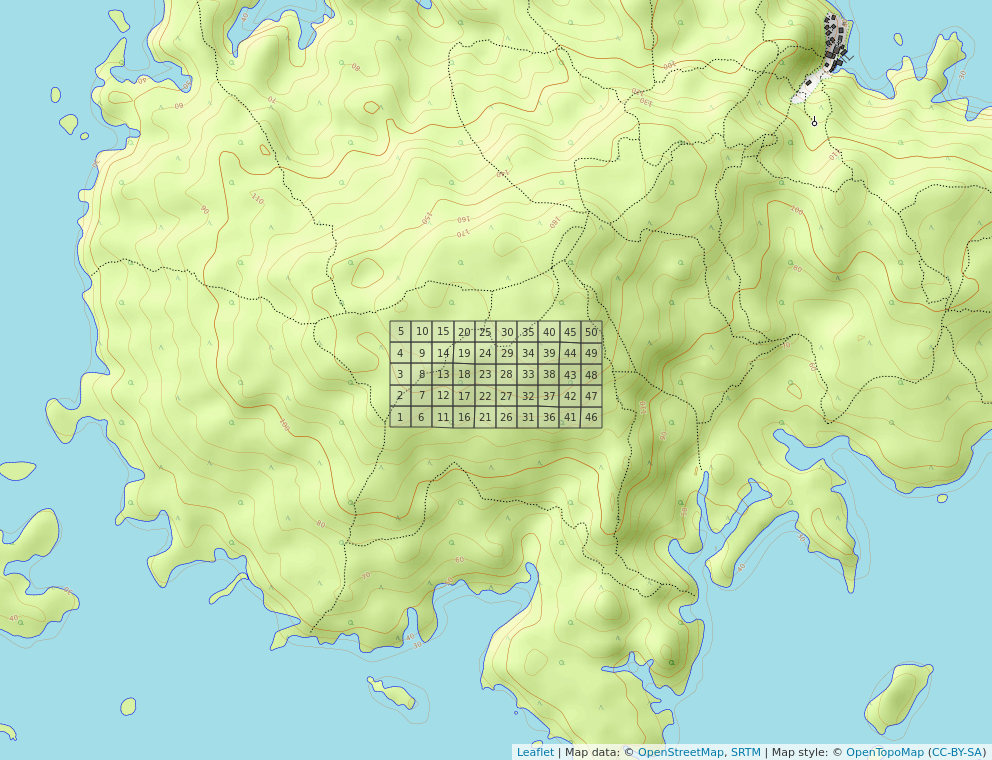
\includegraphics[width=1.00000\textwidth]{mapa_cuadros2.png}
\caption{Mapa de la Isla Barro Colorado y la parcela
permante\label{fig:bci_map}}
\end{figure}

\section{Metodología y materiales}\label{metodologuxeda-y-materiales}

Para el estudio de la biodiversidead de la familia \emph{Myrtaceae} se
usaron los datos censales de las 50 parcelas forestales de \emph{BCI}
que están presentes en el repositorio \texttt{scripts-de-analisis-BCI}
(Batlle, 2020), de los cuales fueron tratados y procesados con distintos
algoritmos y técnicas de medición, cálculo, análisis e interpretación
por medio del entorno de desarrollo intregado y libre, \emph{RStudio} (R
Core Team, 2020). En cuanto a los gráficos presentes se obtuvieron por
medio \emph{R}, usando paquetes y funciones (ver
tabla\ref{tab:materiales}).

Para iniciar los análisis estadísticos de datos con dimensiones
diversas, Buzai \& Baxendale (2009) y Borcard et al. (2011), recomiendan
realizar un análisis exploratorio de datos (EDA), debido a que es una
herramienta imprescindible para conseguir una primera inmediación,
información genérica de los datos, realizar transformaciones a variables
de ser necesarias, y poder conducir más análisis. Se usaron los paquetes
\texttt{vegan}, \texttt{tidyverse}, \texttt{sf}, \texttt{mapview} y
\texttt{RColorBrewer} para cargar los datos censales, matriz de
comunidad y matriz ambiental, y así poder extraer los datos de la
familia \emph{Myrtaceae}, de las variables ambientales y transformarlos
en tablas, matrices, e incluso generar gráficos de mapas. También, se
usaron las librerías \texttt{psych} y \texttt{ez}, en conjunto con las
anteriores para ver correlaciones de la \emph{Myrtaceae} con distintas
variables ambientales con la función \texttt{cor}, y generar mapas de
variables ambientales por cada cuadro con \texttt{ggplot2}.

La medida de los coeficientes de asociación de la familia
\emph{Myrtaceae} con los modos \emph{Q} y \emph{R} {[}{]} se realizó
mediante funciones pertenecientes a las librerias \texttt{vegan},
\texttt{adespatial}, \texttt{broom}, \texttt{tidyverse}, \texttt{sf},
\texttt{cluster} y \texttt{gclus}. En el modo \emph{Q} se mide la
abundancia de las especies de \emph{Myrtaceae} con la función
\texttt{dist.ldc} que calcula la distancia euclidea entre dos sitios y
se usa también el método de transformación \emph{Hellinger} {[}{]} y asi
obtener el grado de disimilaridad entre sitios. También, se calculó la
distancia de \emph{Jaccard} \emph{Dj} {[}{]} utilizando la función
\texttt{vegdist} que convierte la matriz de comunidad en una de
presencia/ausencia para calcular la matriz de distancia. En cuanto a la
asociación de las variables ambientales, se hizo un nuevo ambiente con
la función \texttt{env} para las variables transfomardas con la función
\texttt{scale}. De igual manera, se usó la función \texttt{env\_mix}
para asociar las variables ambientales heterogeneidad ambiental, hábitat
y quebrada, generando una matriz de disimilaridad.

Con el modo \emph{R} de medición de asociación, se mensuró el grado de
asociación entre especies haciendo una transformación de la matriz de
comunidad usando la estandarización \emph{Chi} con la función
\texttt{decostand}, luego se calcula la distancia con la función
\texttt{dist} y se reresenta la matriz en un mapa de calor con la
función \texttt{coldiss}. Se calculó la distancia de \emph{Jaccard}
{[}{]} entre especies usando la matriz de comunidad transpuesta
convertida a una de presencia/ausencia con la función \texttt{vegdist}.
En cuanto a la asociación de variables ambientales númericas, usando el
índice de \emph{rho} de \emph{Spearman} {[}{]} con los verbos
\texttt{select}, \texttt{mutate} y \texttt{matches} de la herramienta
\texttt{dplyr} y también la función \texttt{cor} para correlación.

Los análisis de agrupamiento o cluster análisis aplicados a la familia
\emph{Myrtaceae} fueron realizados usando las librerías
\texttt{magrittr}, \texttt{broom}, \texttt{tidyverse}, \texttt{mapview}
y \texttt{indicspecies}. Para el estudio se usó el agrupamiento
jerárquico (\emph{AJ}) con un enfoque aglomerativo por enlace simple
{[}{]}, completo {[}{]}, promedio {[}{]} y el método de \emph{Ward} de
varianza mínima {[}{]}. Se agruparon pares de objetos según la mayor
similaridad (vecino más próximo o mínima distancia), partiendo del
agrupamiento por enlace simple, utilizando la matriz de comunidad
transformada por medio del método de normalización con la función
\texttt{decostand} y la distancia euclidea con la función
\texttt{vegdist}. El agrupamiento jerárquico se hizo conn la función
\texttt{hclust} para método simple y se generó un dendrograma (gráfico)
con la función \texttt{plot} del resultado de este AJ. Para el
agrupamiento completo usando la menor similaridad (máxima distancia o
vecino más lejano) se empleó la función \texttt{hclust} y la matriz de
distancia de cuerdas o \emph{chord} {[}{]}, con tal de generar un
dendrograma con la función \texttt{plot}. En cuanto al agrupamiento por
enlace promedio (UPGMA, WPGMA, UPGMC, WPGMC), se usó el UPGMA {[}{]},
para máximizar la correlación entre las distancias cofenética
(coeficiente de correlación de Pearson), para esto se usó la función
\texttt{hclust} y para obtener el gráfico la función \texttt{plot}.
Finalmente, el agrupamiento por Ward {[}{]}, que define los grupos de
una forma donde la suma de cuadrados se minimice en cada uno de ellos
usando las funciones \texttt{hclust} y \texttt{plot}.

De todos los metodos anteriores de agrupamiento, se han seleccionado
ideal para la familia \emph{Myrtaceae} se usó la función \texttt{map} y
así coparar sus valores. Además, para la elección del número de clusters
se usó la función \texttt{calcular\_anchuras\_siluetas} en base a la
matriz de comunidad original, la matriz de distancias y objeto de
clúster usando UPGMA y Ward, luego, se hizo un nuevo dengrama con la
función \texttt{reorder.hclust} y un mapa de calor con la función
\texttt{heatmap}. Finalmente, se hizo una evaluación para ver si el
número de clusters obtenidos por los métodos anteriores son los ideales
usando el método \emph{bootstrap} {[}{]}, usando el paquete
\texttt{pvclust} para generar dendogramas con trazos en rectangulos y
lineas que dividen el gráfico acorde al número de grupos.

En cuanto al agrupamiento de variables se usaron los grupos obtenidos
por UPGMA para evaluar la homogeneidad por medio de pruebas \emph{t}
{[}{]}, basadas en la distribución \emph{t} de \emph{Student} {[}{]} y
la suma de rangos de \emph{Wilcoxon} {[}{]}, a partir de esto se
generaron gráficos de caja y mapas presentando la ubicación por cuadrado
de cada grupo en la parcela permanente. Y para la homogeneidad de los
grupos Ward se usó el método ANOVA {[}{]} y Kruskal/Wallis {[}{]}.

Cerrando con el clusters análisis, se obtuvieron las especies
indicadoras y las especies con preferencias por hábitats; la primera
mediante \texttt{IndVal} con las funciones \texttt{multipatt} y
\texttt{strassoc} y su significancia o valor p con la función
\texttt{p.adjust}; las especies con preferencias por hábitats se
obtuvieron mediante el coeficiente de correlación biserial puntual
{[}{]} con las funciones \texttt{multipatt} y \texttt{strassoc}.

\section{Resultados}\label{resultados}

Ver tabla \ref{tab:abun_sp} y figura \ref{fig:abun_sp_q}

\section{Discusión}\label{discusiuxf3n}

\section{Agradecimientos}\label{agradecimientos}

\section{Información de soporte}\label{informaciuxf3n-de-soporte}

\begin{longtable}[]{@{}cc@{}}
\caption{\label{tab:materiales} Materiales usados en el
estudio}\tabularnewline
\toprule
\begin{minipage}[b]{0.14\columnwidth}\centering\strut
Materiales\strut
\end{minipage} & \begin{minipage}[b]{0.80\columnwidth}\centering\strut
Uso\strut
\end{minipage}\tabularnewline
\midrule
\endfirsthead
\toprule
\begin{minipage}[b]{0.14\columnwidth}\centering\strut
Materiales\strut
\end{minipage} & \begin{minipage}[b]{0.80\columnwidth}\centering\strut
Uso\strut
\end{minipage}\tabularnewline
\midrule
\endhead
\begin{minipage}[t]{0.14\columnwidth}\centering\strut
RStudio\strut
\end{minipage} & \begin{minipage}[t]{0.80\columnwidth}\centering\strut
Redacción del manuscrito, procesamientos de datos censales de la familia
\emph{Myrtaceae} por medio de Scripts.\strut
\end{minipage}\tabularnewline
\begin{minipage}[t]{0.14\columnwidth}\centering\strut
library vegan\strut
\end{minipage} & \begin{minipage}[t]{0.80\columnwidth}\centering\strut
Conjunto de herramientas para hacer análisis de diversidad, ordenación
de comunidad y análisis de disimilaridad.\strut
\end{minipage}\tabularnewline
\begin{minipage}[t]{0.14\columnwidth}\centering\strut
library tidiyverse\strut
\end{minipage} & \begin{minipage}[t]{0.80\columnwidth}\centering\strut
Colección de paquetes que permiten transformar, importar, visualizar,
modelar y presentar distintos datos.\strut
\end{minipage}\tabularnewline
\begin{minipage}[t]{0.14\columnwidth}\centering\strut
library sf\strut
\end{minipage} & \begin{minipage}[t]{0.80\columnwidth}\centering\strut
Creación de simple features, ampliando objetos tipo data.frame con una
columna de lista de características simples.\strut
\end{minipage}\tabularnewline
\begin{minipage}[t]{0.14\columnwidth}\centering\strut
library mapview\strut
\end{minipage} & \begin{minipage}[t]{0.80\columnwidth}\centering\strut
Para ver objetos espaciales de forma interactiva sobre un mapa
base.\strut
\end{minipage}\tabularnewline
\begin{minipage}[t]{0.14\columnwidth}\centering\strut
library RColorBrewer\strut
\end{minipage} & \begin{minipage}[t]{0.80\columnwidth}\centering\strut
Para crear paletas de colores para mapas temáticos.\strut
\end{minipage}\tabularnewline
\begin{minipage}[t]{0.14\columnwidth}\centering\strut
library ez\strut
\end{minipage} & \begin{minipage}[t]{0.80\columnwidth}\centering\strut
Permiten una visualización y análisis de datos simples y con
especificaciones consistentes.\strut
\end{minipage}\tabularnewline
\begin{minipage}[t]{0.14\columnwidth}\centering\strut
library psych\strut
\end{minipage} & \begin{minipage}[t]{0.80\columnwidth}\centering\strut
Conjunto de herramientas para hacer análisis de datos
multivariados.\strut
\end{minipage}\tabularnewline
\begin{minipage}[t]{0.14\columnwidth}\centering\strut
library tmap\strut
\end{minipage} & \begin{minipage}[t]{0.80\columnwidth}\centering\strut
Para visualizar, con mapas temáticos, la distribución de datos
espaciales.\strut
\end{minipage}\tabularnewline
\begin{minipage}[t]{0.14\columnwidth}\centering\strut
library adespatial\strut
\end{minipage} & \begin{minipage}[t]{0.80\columnwidth}\centering\strut
Herramienta para hacer análisis espaciales, a distintas escalas, de
datos multivariados.\strut
\end{minipage}\tabularnewline
\begin{minipage}[t]{0.14\columnwidth}\centering\strut
library broom\strut
\end{minipage} & \begin{minipage}[t]{0.80\columnwidth}\centering\strut
Para resumir información de objetos estadísticos en tablas.\strut
\end{minipage}\tabularnewline
\begin{minipage}[t]{0.14\columnwidth}\centering\strut
library cluster\strut
\end{minipage} & \begin{minipage}[t]{0.80\columnwidth}\centering\strut
Para el clúster análisis o de agrupamiento, que permiten encontrar
grupos de datos.\strut
\end{minipage}\tabularnewline
\begin{minipage}[t]{0.14\columnwidth}\centering\strut
library gclus\strut
\end{minipage} & \begin{minipage}[t]{0.80\columnwidth}\centering\strut
Ordena en matrices de diagramas, dispersión y coordenadas paralelas con
un índice, los paneles.\strut
\end{minipage}\tabularnewline
\begin{minipage}[t]{0.14\columnwidth}\centering\strut
library magittr\strut
\end{minipage} & \begin{minipage}[t]{0.80\columnwidth}\centering\strut
Paquete que permite, mediante mecanismos, cadenas de comandos con el
operador pipa.\strut
\end{minipage}\tabularnewline
\begin{minipage}[t]{0.14\columnwidth}\centering\strut
library pvclust\strut
\end{minipage} & \begin{minipage}[t]{0.80\columnwidth}\centering\strut
Paquete que permite implementar un remuestreo multiescala para evaluar
inconsistencia en análisis de agrupamiento jerárquico.\strut
\end{minipage}\tabularnewline
\begin{minipage}[t]{0.14\columnwidth}\centering\strut
library indicspecies\strut
\end{minipage} & \begin{minipage}[t]{0.80\columnwidth}\centering\strut
Estima el valor estadístico de la relación presencia-abundancia de
especies y sus sitios.\strut
\end{minipage}\tabularnewline
\begin{minipage}[t]{0.14\columnwidth}\centering\strut
library plyr\strut
\end{minipage} & \begin{minipage}[t]{0.80\columnwidth}\centering\strut
Conjunto de herramientas que permiten separar, aplicar y combinar datos
para generar resúmenes estadísticos de ellos.\strut
\end{minipage}\tabularnewline
\begin{minipage}[t]{0.14\columnwidth}\centering\strut
library SpadeR\strut
\end{minipage} & \begin{minipage}[t]{0.80\columnwidth}\centering\strut
Estima diversos índices de biodiversidad y medidas de similitud de datos
individuales tomados de diversas comunidades.\strut
\end{minipage}\tabularnewline
\begin{minipage}[t]{0.14\columnwidth}\centering\strut
library iNEXT\strut
\end{minipage} & \begin{minipage}[t]{0.80\columnwidth}\centering\strut
Paquete que permite calcular y trazar la rarefacción y extrapolación de
diversidad de especies.\strut
\end{minipage}\tabularnewline
\begin{minipage}[t]{0.14\columnwidth}\centering\strut
library vegetarian\strut
\end{minipage} & \begin{minipage}[t]{0.80\columnwidth}\centering\strut
Para calcular la diversidad por comunidad en un conjunto de datos.\strut
\end{minipage}\tabularnewline
\begin{minipage}[t]{0.14\columnwidth}\centering\strut
library ape\strut
\end{minipage} & \begin{minipage}[t]{0.80\columnwidth}\centering\strut
Paquete que permite hacer análisis filogenéticos y evolutivos de
árboles.\strut
\end{minipage}\tabularnewline
\begin{minipage}[t]{0.14\columnwidth}\centering\strut
library spdep\strut
\end{minipage} & \begin{minipage}[t]{0.80\columnwidth}\centering\strut
Conjunto de funciones para crear matrices de ponderaciones espaciales de
puntos de patrones polígonos, entre otros.\strut
\end{minipage}\tabularnewline
\begin{minipage}[t]{0.14\columnwidth}\centering\strut
library ade4\strut
\end{minipage} & \begin{minipage}[t]{0.80\columnwidth}\centering\strut
Herramientas para análisis de datos multivariados.\strut
\end{minipage}\tabularnewline
\begin{minipage}[t]{0.14\columnwidth}\centering\strut
library adegraphics\strut
\end{minipage} & \begin{minipage}[t]{0.80\columnwidth}\centering\strut
Sirve para hacer representaciones gráficas de datos multivariados.\strut
\end{minipage}\tabularnewline
\begin{minipage}[t]{0.14\columnwidth}\centering\strut
library gridExtra\strut
\end{minipage} & \begin{minipage}[t]{0.80\columnwidth}\centering\strut
Ofrece funciones para poder trabajar con gráficos en \emph{grid} y crear
diversos trazados en una página y dibujar tablas.\strut
\end{minipage}\tabularnewline
\begin{minipage}[t]{0.14\columnwidth}\centering\strut
library grid\strut
\end{minipage} & \begin{minipage}[t]{0.80\columnwidth}\centering\strut
Reescribe los gráficos, sus capacidades y da soporte a la
interacción.\strut
\end{minipage}\tabularnewline
\begin{minipage}[t]{0.14\columnwidth}\centering\strut
library gtable\strut
\end{minipage} & \begin{minipage}[t]{0.80\columnwidth}\centering\strut
Herramientas que permiten trabajar más fácil con tablas.\strut
\end{minipage}\tabularnewline
\bottomrule
\end{longtable}

\section{\texorpdfstring{\emph{Script}
reproducible}{Script reproducible}}\label{script-reproducible}

\ldots

\section*{Referencias}\label{referencias}
\addcontentsline{toc}{section}{Referencias}

\hypertarget{refs}{}
\hypertarget{ref-sandra2019myrtaceae}{}
Almeida, S. (2019). \emph{Myrtaceae, familia}. Retrieved from
\url{https://knoow.net/es/ciencias-tierra-vida/biologia-es/myrtaceae-familia/}

\hypertarget{ref-jose_ramon_martinez_batlle_2020_4402362}{}
Batlle, J. R. M. (2020). biogeografia-master/scripts-de-analisis-BCI:
Long coding sessions (Version v0.0.0.9000).
\url{https://doi.org/10.5281/zenodo.4402362}

\hypertarget{ref-borcard2011numerical}{}
Borcard, D., Gillet, F., Legendre, P., \& others. (2011).
\emph{Numerical ecology with r} (Vol. 2). Springer.

\hypertarget{ref-encymyrtaceae}{}
Britannica, E. (2016). \emph{Myrtaceae}. Retrieved from
\url{https://www.britannica.com/plant/Myrtaceae}

\hypertarget{ref-buzai2009analisis}{}
Buzai, G. D., \& Baxendale, C. A. (2009). Análisis exploratorio de datos
espaciales. \emph{Geografía Y Sistemas de Información Geográfica, No
1,(2009)}.

\hypertarget{ref-claver1984guia}{}
Claver Farías, I., \& others. (1984). Guía para la elaboración de
estudios del medio físico: Contenido y metodología. \emph{Ministerio de
Obras Públicas Y Urbanismo. Madrid}.

\hypertarget{ref-de2003ecologia}{}
De la Llata Loyola, M. D. (2003). \emph{Ecología y medio ambiente}.
Editorial Progreso.

\hypertarget{ref-Hubbell2005barro}{}
Hubbell, S., Foster, R., \& Condit, R. (2005). \emph{Barro colorado
forest census plot data}. Retrieved from
\url{http://ctfs.si.edu/webatlas/datasets/bci/}

\hypertarget{ref-legendre2012numerical}{}
Legendre, P., \& Legendre, L. (2012). \emph{Numerical ecology}.
Elsevier.

\hypertarget{ref-josemyrtaceae}{}
Lorenzo-Cáceres, J. M. S. de. (s.f.). \emph{Familia myrtaceae}.
Retrieved from \url{https://www.arbolesornamentales.es/Myrtaceae.htm}

\hypertarget{ref-magurran1988ecological}{}
Magurran, A. E. (1988). \emph{Ecological diversity and its measurement}.
Princeton university press.

\hypertarget{ref-pereztree}{}
Perez, R., \& R, C. (s.f.). \emph{Tree atlas of panama}. Retrieved from
\url{http://ctfs.si.edu/PanamaAtlas/famdescr.php?Family=Myrtaceae}

\hypertarget{ref-perez2005metodologia}{}
Pérez, R., Aguilar, S., Condit, R., Foster, R., Hubbell, S., \& Lao, S.
(2005). Metodologia empleada en los censos de la parcela de 50 hectareas
de la isla de barro colorado, panamá. \emph{Centro de Ciencias
Forestales Del Tropico (CTFS) Y Instituto Smithsonian de Investigaciones
Tropicales (STRI)}, 1--24.

\hypertarget{ref-pineda2014analisis}{}
Pineda, P. (2014). \emph{Análisis del sistema de parcelas permanentes de
medición en los bosques de guatemala. informe final}. Guatemala:
Proyecto" Sistemas de información sobre la productividad de
los~\ldots{}.

\hypertarget{ref-R2020ALanguage}{}
R Core Team. (2020). \emph{R: A language and environment for statistical
computing}. Retrieved from \url{https://www.R-project.org/}

\hypertarget{ref-rodriguez2021colonizacion}{}
Rodríguez-Castro, L., \& Flores, N. (2021). Colonización de la hepática
epífila leptolejeunea elliptica (lehm \& lindenb)
schiffn.(Lejeuneaceae), sobre dos especies de arbustos de la isla barro
colorado (bci). \emph{Tecnociencia}, \emph{23}(1), 82--103.

\hypertarget{ref-sugasti2018medicion}{}
Sugasti, L., Eng, B., \& Pinzón, R. (2018). Medición continúa de flujo
de co2 ensuelo en una parcela de bosque tropical en isla barro colorado,
canal de panamá. \emph{Universidad Tecnológica de Panamá}, 1--7.

\hypertarget{ref-whittaker1972evolution}{}
Whittaker, R. H. (1972). Evolution and measurement of species diversity.
\emph{Taxon}, \emph{21}(2-3), 213--251.




\newpage
\singlespacing 
\end{document}
